% Standalone architecture figure for the passive shared-technician proposal.
\documentclass[tikz,border=6pt]{standalone}
\usepackage{amsmath}
\usepackage{tikz}
\usetikzlibrary{arrows.meta,backgrounds,calc,fit,positioning}

\definecolor{agentblue}{HTML}{DCEAF7}
\definecolor{resourceorange}{HTML}{F8E6CF}
\definecolor{envgray}{HTML}{F1F2F2}
\definecolor{feedbackgreen}{HTML}{DCEEDC}
\definecolor{ink}{HTML}{263238}

\tikzset{
  >=Latex,
  line/.style={->, thick, draw=ink},
  feedback/.style={->, thick, dashed, draw=ink},
  panel/.style={draw=ink, rounded corners=2pt, line width=0.8pt},
  agent/.style={panel, fill=agentblue, minimum width=2.15cm, minimum height=0.78cm, align=center},
  resource/.style={panel, fill=resourceorange, minimum width=2.35cm, minimum height=1.00cm, text width=2.10cm, align=center},
  item/.style={panel, fill=white, minimum width=2.35cm, minimum height=1.00cm, text width=2.10cm, align=center},
  heading/.style={font=\small\bfseries, text=ink},
}

\begin{document}
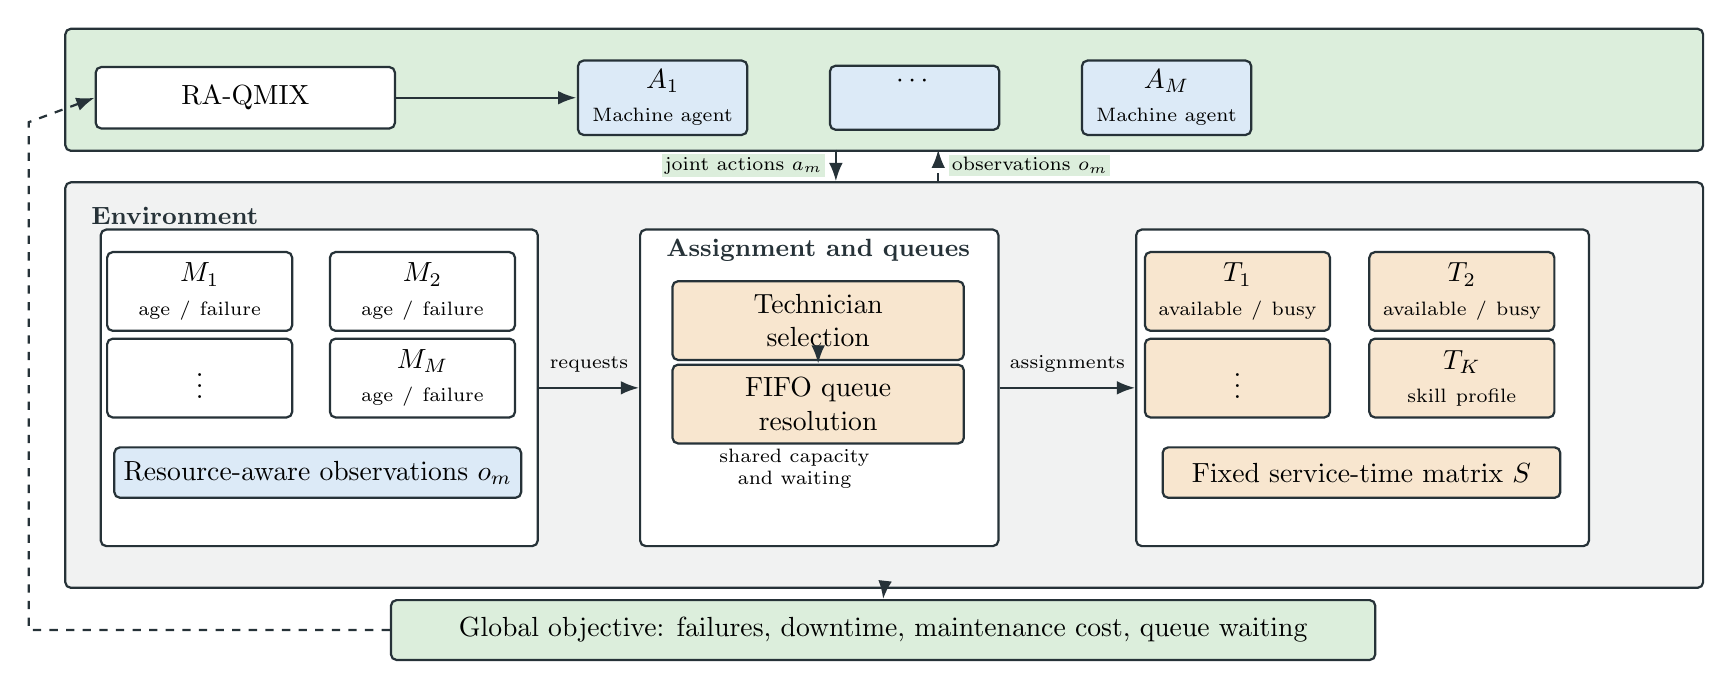
\begin{tikzpicture}[x=1cm,y=1cm]

% Learning and agent layer.
\node[panel, fill=feedbackgreen, minimum width=20.8cm, minimum height=1.55cm,
      anchor=north west] (learning) at (0,0) {};
\node[panel, fill=white, minimum width=3.80cm, minimum height=0.78cm,
      align=center] (algorithm) at (2.30,-0.89)
      {RA-QMIX};
\node[agent] (a1) at (7.60,-0.89) {$A_1$\\\scriptsize Machine agent};
\node[agent] (ai) at (10.80,-0.89) {$\cdots$\\\scriptsize};
\node[agent] (am) at (14.00,-0.89) {$A_M$\\\scriptsize Machine agent};
\node[draw=none, inner sep=0pt, fit=(a1)(ai)(am)] (agentgroup) {};
\draw[line] (algorithm.east) -- (agentgroup.west);

% Environment boundary and title.
\node[panel, fill=envgray, minimum width=20.8cm, minimum height=5.15cm,
      anchor=north west] (environment) at (0,-1.95) {};
\node[heading, anchor=north west] at (0.22,-2.16)
      {Environment};

% Machines column.
\node[panel, fill=white, minimum width=5.55cm, minimum height=4.02cm,
      anchor=north west] (machines) at (0.45,-2.55) {};
\node[heading, anchor=north west] at (0.68,-2.74)
      {Machines};
\node[item] (m1) at (1.72,-3.35) {$M_1$\\\scriptsize age / failure};
\node[item] (m2) at (4.55,-3.35) {$M_2$\\\scriptsize age / failure};
\node[item] (mm) at (1.72,-4.45) {$\vdots$};
\node[item] (mM) at (4.55,-4.45) {$M_M$\\\scriptsize age / failure};
\node[panel, fill=agentblue, minimum width=5.05cm, minimum height=0.64cm,
      align=center] (obs) at (3.22,-5.65)
      {Resource-aware observations $o_m$};

% Assignment/queue column.
\node[panel, fill=white, minimum width=4.55cm, minimum height=4.02cm,
      anchor=north west] (dispatch) at (7.30,-2.55) {};
\node[heading, align=center] at (9.575,-2.83)
      {Assignment and queues};
\node[panel, fill=resourceorange, minimum width=3.70cm, minimum height=1.00cm,
      text width=3.35cm, align=center] (assign) at (9.575,-3.72)
      {Technician\\selection};
\node[panel, fill=resourceorange, minimum width=3.70cm, minimum height=1.00cm,
      text width=3.35cm, align=center] (fifo) at (9.575,-4.78)
      {FIFO queue\\resolution};
\draw[line] (assign) -- (fifo);
\node[font=\scriptsize, align=center] at (9.275,-5.60)
      {shared capacity\\and waiting};

% Technician column.
\node[panel, fill=white, minimum width=5.75cm, minimum height=4.02cm,
      anchor=north west] (technicians) at (13.60,-2.55) {};
\node[heading, anchor=north west] at (13.83,-2.74)
      {Technicians};
\node[resource] (t1) at (14.90,-3.35) {$T_1$\\\scriptsize available / busy};
\node[resource] (t2) at (17.75,-3.35) {$T_2$\\\scriptsize available / busy};
\node[resource] (tk) at (14.90,-4.45) {$\vdots$};
\node[resource] (tK) at (17.75,-4.45) {$T_K$\\\scriptsize skill profile};
\node[panel, fill=resourceorange, minimum width=5.05cm, minimum height=0.64cm,
      align=center] (service) at (16.475,-5.65)
      {Fixed service-time matrix $S$};

% Environment flow.
\draw[line] (machines.east) -- node[above, font=\scriptsize, yshift=2pt] {requests} (dispatch.west);
\draw[line] (dispatch.east) -- node[above, font=\scriptsize, yshift=2pt] {assignments} (technicians.west);
\draw[line] (9.80,-1.55) -- (9.80,-1.95);
\node[font=\scriptsize, anchor=east, fill=feedbackgreen, inner sep=1pt] at (9.67,-1.75)
      {joint actions $a_m$};
\draw[feedback] (11.10,-1.95) -- (11.10,-1.55);
\node[font=\scriptsize, anchor=west, fill=feedbackgreen, inner sep=1pt] at (11.23,-1.75)
      {observations $o_m$};

% Objective and feedback.
\node[panel, fill=feedbackgreen, minimum width=12.5cm, minimum height=0.76cm,
      align=center] (objective) at (10.40,-7.65)
      {Global objective: failures, downtime, maintenance cost, queue waiting};
\draw[line] (environment.south) -- (objective.north);
\draw[feedback] (objective.west) -- (-0.45,-7.65) -- (-0.45,-1.20) -- (algorithm.west);

\end{tikzpicture}
\end{document}
